%section 7
%%%%%%%%%%%%%%%%%%%%%%%%%%%%%%%%%%%%%%%
%%%%%%%%%%%%%%%%%%%%%%%%%%%%%%%%%%%%%%%

\section{図表}
駒場の実験で、レポートにおける図や表の貼り方を教わったと思います。図は下
に、表は上にキャプションをつけるのでした。また、図や表を貼ったら\emph{必
ず}本文中で説明する必要があります。このとき「図~3より」とか「表~127より」
というように番号を参照しますが、これを手動でやっていたらまあそのうち番号
がおかしくなるはずです。{\LaTeX}ではこの作業を自動で行えるようになってい
ます。

本節ではまず表の書き方、図の貼り方を説明したあと、参照の仕方を説明します。

\subsection{表の書き方}\label{sub:tabular}
表を書くにはtabular環境を使います。使い方は
\begin{screen}
\verb+\begin{tabular}{列指定子}+ \\
$\begin{array}{cccccc}
 a_{1,1} & \verb+&+ & \cdots & \verb+&+ & a_{1,n} & \verb+\\+ \\
 \vdots  & \verb+&+ & \ddots & \verb+&+ & \vdots  & \verb+\\+ \\
 a_{m,1} & \verb+&+ & \cdots & \verb+&+ & a_{m,n} &
\end{array}$\\
\verb+\end{tabular}+
\end{screen}
です。先に出てきたarray環境と似ていますね。というか、数式環境に入
れなくてよいことを除けばarray環境とまったく同じです。
ですから、基本的な使い方は次のようになります。\\
\begin{minipage}[c]{.50\textwidth}
\begin{screen}
\small
\begin{verbatim}
\begin{tabular}{lll}
 l & 左寄せ  & Leftの略   \\
 c & 中央    & Centerの略 \\
 r & 右寄せ  & Rightの略
\end{tabular}
\end{verbatim}
\end{screen}
\end{minipage}%
%\manerrarrow\hfill{}
$\Rightarrow$
\begin{minipage}{.45\textwidth}
\begin{shadebox}
\begin{tabular}{lll}
 l & 左寄せ  & Leftの略   \\
 c & 中央    & Centerの略 \\
 r & 右寄せ  & Rightの略
\end{tabular}
\end{shadebox}
\end{minipage}
\vspace*{1mm}\\
\begin{minipage}[c]{.50\textwidth}
\begin{screen}
\small
\begin{verbatim}
\begin{tabular}{||c|c|c||}
 l & 左寄せ  & Leftの略   \\
 c & 中央    & Centerの略 \\
 r & 右寄せ  & Rightの略
\end{tabular}
\end{verbatim}
\end{screen}
\end{minipage}%
%\manerrarrow\hfill{}
$\Rightarrow$
\begin{minipage}{.45\textwidth}
\begin{shadebox}
\begin{tabular}{||c|c|c||}
 l & 左寄せ  & Leftの略   \\
 c & 中央    & Centerの略 \\
 r & 右寄せ  & Rightの略
\end{tabular}
\end{shadebox}
\end{minipage}
\vspace*{1mm}\\
横方向の罫線を引くには、表\ref{tab:rule}に示したような命令を使います。
\begin{table}[htbp]
\begin{center}
\caption{主な罫線命令}
\label{tab:rule}
\begin{tabular}{ll}
\hline
命令 & 意味 \\
\hline
\verb+\hline+             & 横に引けるだけの罫線を引く     \\
\verb+\hline\hline+  & 横に引けるだけの二重罫線を引く \\
\verb+\vline+             & 引けるだけの縦罫線を引く       \\
\verb+\cline{範囲}+    & 横罫線を列の範囲を指定して引く \\
\verb+\multicolumn{数値}{列指定子}{要素}+ &
                          行をつなげて列指定子どおりに要素を出力する \\
\hline
\end{tabular}
\end{center}
\end{table}

使用例を考察していきましょう。
\verb+\hline+,\verb+\hline\hline+,\verb+\vline+は簡単です。\\
\begin{minipage}[c]{.50\textwidth}
\begin{screen}
\small
\begin{verbatim}
\begin{tabular}{lll}\hline\hline
 l & 左寄せ  & Leftの略   \\
\hline
 c & 中央    & Center\vline の略 \\
\hline
 r & 右寄\vline せ  & Rightの略  \\
\hline\hline
\end{tabular}
\end{verbatim}
\end{screen}
\end{minipage}%
%\manerrarrow\hfill{}
$\Rightarrow$
\begin{minipage}{.45\textwidth}
\begin{shadebox}
\begin{tabular}{lll}\hline\hline
 l & 左寄せ  & Leftの略   \\
\hline
 c & 中央    & Center\vline の略 \\
\hline
 r & 右寄\vline せ  & Rightの略  \\
\hline\hline
\end{tabular}
\end{shadebox}
\end{minipage}
\vspace*{1mm}\\
\verb+\vline+は使いどころが難しいようですね。\verb+\cline+はこんなふうに使い
ます。\\
\begin{minipage}[c]{.50\textwidth}
\begin{screen}
\small
\begin{verbatim}
\begin{tabular}{lll}\hline\hline
 l & 左寄せ  & Leftの略   \\
\cline{1-1}
 c & 中央    & Centerの略 \\
\cline{2-3}
 r & 右寄せ  & Rightの略  \\
\hline\hline
\end{tabular}
\end{verbatim}
\end{screen}
\end{minipage}%
%\manerrarrow\hfill{}
$\Rightarrow$
\begin{minipage}{.45\textwidth}
\begin{shadebox}
\begin{tabular}{lll}\hline\hline
 l & 左寄せ  & Leftの略   \\
\cline{1-1}
 c & 中央    & Centerの略 \\
\cline{2-3}
 r & 右寄せ  & Rightの略  \\
\hline\hline
\end{tabular}
\end{shadebox}
\end{minipage}
\vspace*{1mm}\\
\verb+\multcolumn+はその名のとおり、列をつなげることができます。\verb+{数値}+
にはつなげる列の数を記入します。まあこんな感じです。\\
\begin{minipage}[c]{.50\textwidth}
\begin{screen}
\small
\begin{verbatim}
\begin{tabular}{|c|c|c|}\hline
\multicolumn{3}{|c|}{列指定子の意味} \\
\hline
 l & 左寄せ  & Leftの略   \\
\hline
 c & 中央    & Centerの略 \\
\hline
 r & 右寄せ  & Rightの略  \\
\hline
\end{tabular}
\end{verbatim}
\end{screen}
\end{minipage}%
%\manerrarrow\hfill{}
$\Rightarrow$
\begin{minipage}{.45\textwidth}
\begin{shadebox}
\begin{tabular}{|c|c|c|}\hline
\multicolumn{3}{|c|}{列指定子の意味} \\
\hline
 l & 左寄せ  & Leftの略   \\
\hline
 c & 中央    & Centerの略 \\
\hline
 r & 右寄せ  & Rightの略  \\
\hline
\end{tabular}
\end{shadebox}
\end{minipage}
\vspace*{1mm}\\
\verb+\multcolumn+はつなげる列の数に\{1\}を入れて、その部分だけ列指定
子を変更することもできます。

全部使えば、これくらいはできます。\\
\begin{minipage}[c]{.50\textwidth}
\begin{screen}
\small
\begin{verbatim}
\begin{tabular}{|c|c|c|c|}\hline
\multicolumn{3}{|l|}{ } & ヨ \\
\cline{2-2}
   & い & \multicolumn{2}{l|}{} \\
\cline{4-4}
\multicolumn{2}{|l|}{} &
\multicolumn{2}{l|}{} \\
\cline{1-1}
\multicolumn{1}{l|}{め} & & ろ &  \\
\cline{3-3}
\multicolumn{2}{|l|}{} &
\multicolumn{2}{l|}{} \\
\cline{1-2}\cline{4-4}
\end{tabular}
\end{verbatim}
\end{screen}
\end{minipage}%
%\manerrarrow\hfill{}
$\Rightarrow$
\begin{minipage}{.45\textwidth}
\begin{shadebox}
\begin{center}
\begin{tabular}{|c|c|c|c|}\hline
\multicolumn{3}{|l|}{ } & ヨ \\
\cline{2-2}
   & い & \multicolumn{2}{l|}{} \\
\cline{4-4}
\multicolumn{2}{|l|}{} &
\multicolumn{2}{l|}{} \\
\cline{1-1}
\multicolumn{1}{l|}{め} & & ろ &  \\
\cline{3-3}
\multicolumn{2}{|l|}{} &
\multicolumn{2}{l|}{} \\
\cline{1-2}\cline{4-4}
\end{tabular}
\end{center}
\end{shadebox}
\end{minipage}
\vspace*{1mm}\\

\subsection{画像ファイルの扱い}\label{sub:image}
画像ファイルの扱い(を説明するの)はなかなか面倒です。というのも、{\LaTeX}
自体には画像ファイルを直接扱う仕組みがないからです。何らかの外部ドライバに
依存することになります。この辺の話はそれなりに面白いので興味のある人は
自分で勉強してください。ここでは非常に天下り的に説明します。

gnuplotなどで作ったeps画像を取り込むには、プリアンブルに
\begin{screen}
\begin{verbatim}
\usepackage[オプション]{graphicx}
\end{verbatim}
\end{screen}
と記述して\verb+graphicx+パッケージを読み込みます。スペルが違うと思うか
もしれませんが、これで正解です。固有名詞なので我慢してください。オ
プションの部分には取り合えずdvipdfmxと書いておくとよいでしょう。

次に画像を貼りたい位置で
\begin{screen}
\begin{verbatim}
\includegraphics[設定]{ファイル名}
\end{verbatim}
\end{screen}
と書きます.[ ]の部分でいろんな設定ができるのですが,とりあえず
``\verb+height=+\mbox{$\langle$}高さ\mbox{$\rangle$}''で高さの設定が、
``\verb+width=+\mbox{$\langle$}幅\mbox{$\rangle$}''で幅の設定ができるということを知
っておけば路頭に迷うことはないでしょう。縦横比は保存されるので、どちら
か片方を書けば十分です。

画像を貼るには手元に貼る画像ファイルを用意し、プロジェクトにアップロードしておくことも必須です。いま、
同じディレクトリにsin.epsという画像ファイルがあったとします。これを
貼るには、以下のようにします。\\
\begin{minipage}[c]{.50\textwidth}
\begin{screen}
\small
\begin{verbatim}
幅50mmで貼るには\\
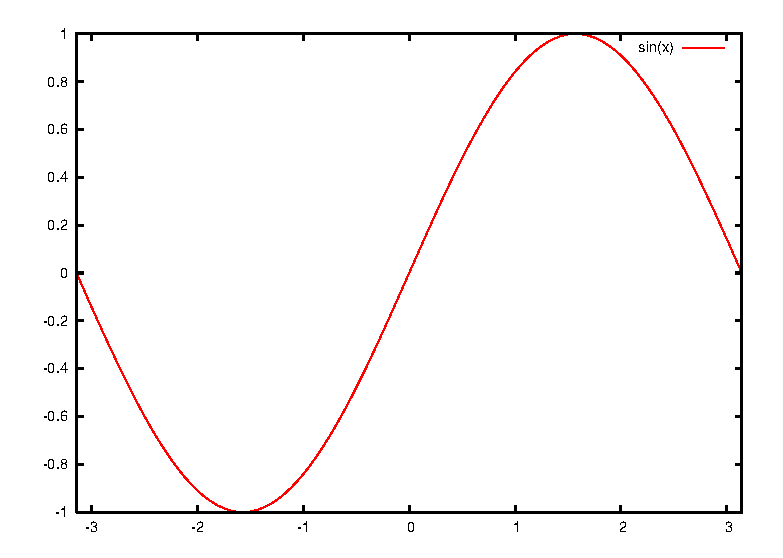
\includegraphics[width=50mm]{sin.eps}\\
これが$\sin x$のグラフです。
\end{verbatim}
\end{screen}
\end{minipage}%
%\manerrarrow\hfill{}
$\Rightarrow$
\begin{minipage}{.45\textwidth}
\begin{shadebox}
幅50mmで貼るには\\
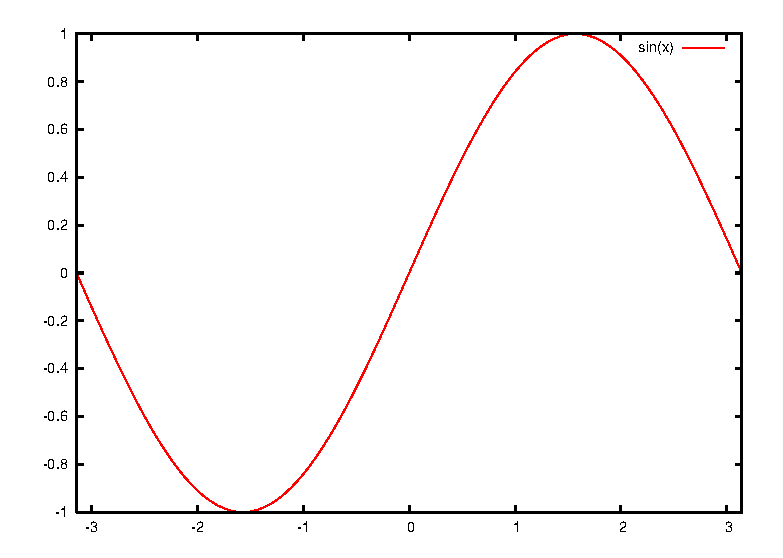
\includegraphics[width=50mm]{sin.eps}\\
これが$\sin x$のグラフです。
\end{shadebox}
\end{minipage}
\vspace*{1mm}\\
\\
\begin{minipage}[c]{.50\textwidth}
\begin{screen}
\small
\begin{verbatim}
高さ20mmで貼るには\\
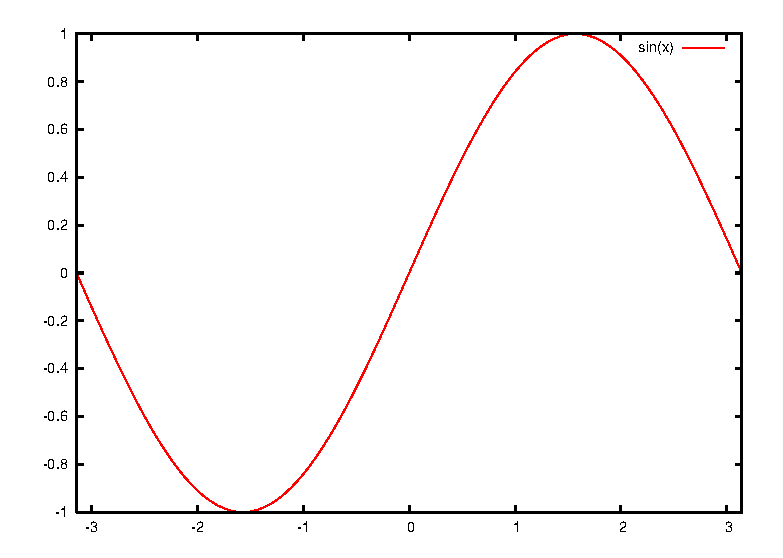
\includegraphics[height=20mm]{sin.eps}\\
これが$\sin x$のグラフです。
\end{verbatim}
\end{screen}
\end{minipage}%
%\manerrarrow\hfill{}
$\Rightarrow$
\begin{minipage}{.45\textwidth}
\begin{shadebox}
高さ20mmで貼るには\\
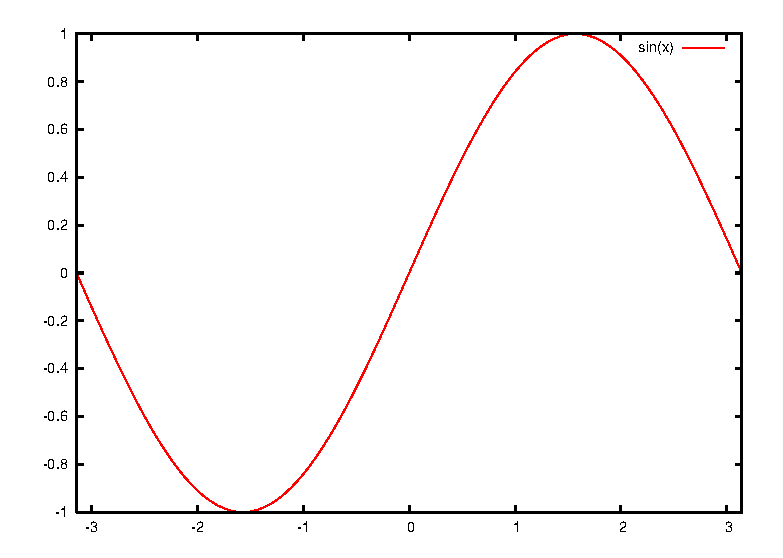
\includegraphics[height=20mm]{sin.eps}\\
これが$\sin x$のグラフです。
\end{shadebox}
\end{minipage}
\vspace*{1mm}\\
\\
\begin{minipage}[c]{.50\textwidth}
\begin{screen}
\small
\begin{verbatim}
縦横比を壊すことも可能です。\\
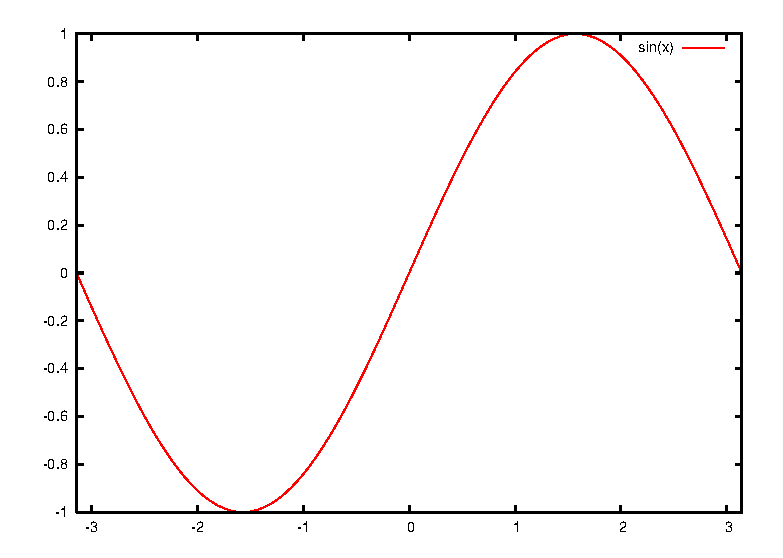
\includegraphics[height=20mm,width=50mm]
{sin.eps}\\
これが$\sin x$のグラフです。
\end{verbatim}
\end{screen}
\end{minipage}%
%\manerrarrow\hfill{}
$\Rightarrow$
\begin{minipage}{.45\textwidth}
\begin{shadebox}
縦横比を壊すことも可能です。\\
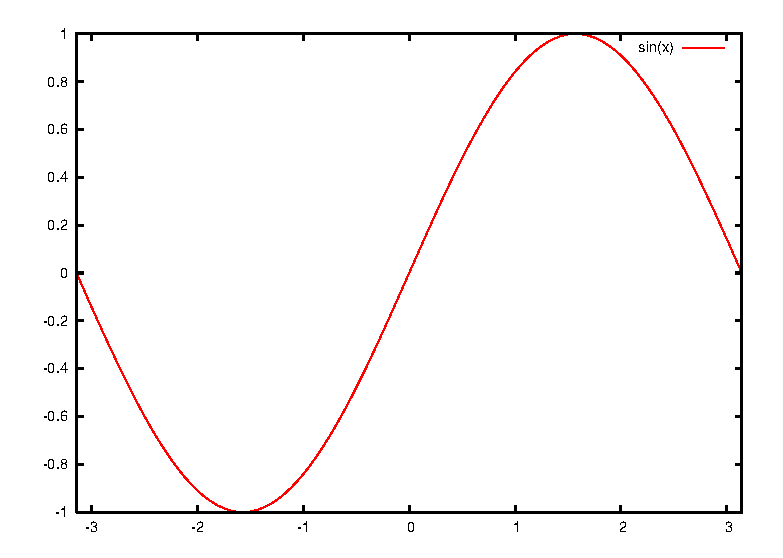
\includegraphics[height=20mm,width=50mm]
{sin.eps}\\
これが$\sin x$のグラフです。
\end{shadebox}
\end{minipage}
\vspace*{1mm}\\
\\
\begin{minipage}[c]{.50\textwidth}
\begin{screen}
\small
\begin{verbatim}
任意の角度だけ図を回転させることも可能です。
ただし角度の単位は\verb+degree+です。\\
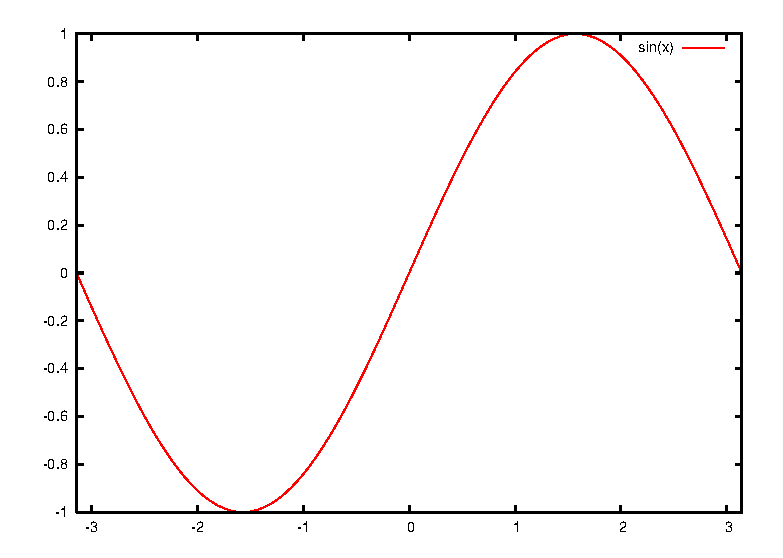
\includegraphics[width=20mm,angle=90.0]
{sin.eps}\\
これが$\sin x$のグラフです。
\end{verbatim}
\end{screen}
\end{minipage}%
%\manerrarrow\hfill{}
$\Rightarrow$
\begin{minipage}{.45\textwidth}
\begin{shadebox}
任意の角度だけ図を回転させることも可能です。
ただし角度の単位は\verb+degree+です。\\
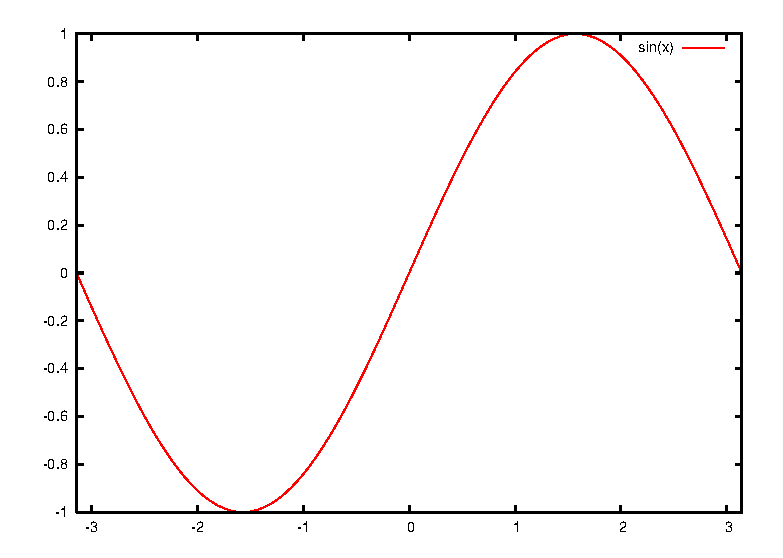
\includegraphics[width=20mm,angle=90.0]
{sin.eps}\\
これが$\sin x$のグラフです。
\end{shadebox}
\end{minipage}
\vspace*{1mm}\\

\subsection{浮動体}
この節の最初に書いたように、図や表の書き方には決まりがあります。これを実
現するために,{\LaTeX}には「浮動体(float)」という概念があります。具体的
には、表を貼り込むときはtable環境で、図を張り込むときはfigure
環境で入れ子にしてやります。こうすることで{\LaTeX}は最適な位置に図や表
を張り込もうとします。図の浮動体の使い方は以下のとおりです。
\begin{screen}
\begin{verbatim}
\begin{figure}[位置指定子]
\includegraphics[設定]{ファイル名}
\caption{図の見出し}
\label{ラベル}
\end{figure}
\end{verbatim}
\end{screen}
一方、表の浮動体の使い方は
\begin{screen}
\begin{verbatim}
\begin{table}[位置指定子]
\caption{表の見出し}
\label{ラベル}
\begin{tabular}
(実際の表本体)
\end{tabular}
\end{table}
\end{verbatim}
\end{screen}
このうち、\verb+\includegraphics+やtabular環境などは
\ref{sub:tabular}節や\ref{sub:image}節で説明したものとまったく
同じです。これを、図ならば\verb+\begin{figure}+と\verb+\end{figure}+で、表
なら\verb+\begin{tabular}+と\verb+\end{tabular}+で囲ってやります。
こうすると、{\LaTeX}はこの図や表のセットを持って移動し、もっとも適切な位
置に出力します。例えばページの下で狭くて入りきらないときは、次のページ
の上のほうに出力しようとするわけです。

ただし、出力位置はある程度はユーザがコントロールすることができます。それが
位置指定子です。位置指定子には表\ref{tab:float}に示すような種類が
あります。
\begin{table}[htbp]
\begin{center}
\caption{浮動体の位置指定子}
\label{tab:float}
\begin{tabular}{cl}
\hline
記号     & 配置する場所           \\
\hline
\verb+h+ & まさにその場所         \\
\verb+t+ & ページの上部           \\
\verb+b+ & ページの下部           \\
\verb+p+ & 新たに別ページをおこす \\
\hline
\end{tabular}
\end{center}
\end{table}
位置指定子を書くことで、図の出力可能位置を指定することができます。
例えば\verb+[htbp]+と書いたりします。何も指定しなければ\verb+[tbp]+
となります。位置指定子は出力可能な場所を指定しているだけなので、htbpを
並べる順番は関係ありません。

\verb+\caption+には図や表のタイトルを記入します。図のタイトルは図の
下、表のタイトルは表の上、という決まりがあるので、図と表では\verb+\caption+
を入力する位置が異なります。

仮に図や表が次のページに旅立っていってしまったとしても、私たちは図や表に
番号が付いているおかげで参照することができます。それが
\verb+\label{ラベル}+の役割です。例えばこのあたりの原稿は次のように書
かれています\footnote{表やグラフを中央揃えにする場合、\verb+\begin{center}+の代わりに\verb+\centering+とする方法もあります。こちらの方が好ましい場合もあります。詳しくは調べてみてください。}。
\begin{screen}
\begin{verbatim}
出力位置は、ある程度はユーザがコントロールすることができます。それが位置指定子です。
位置指定子には表\ref{tab:float}に示すような種類があります。
\begin{table}[htbp]
\begin{center}
\caption{浮動体の位置指定子}
\label{tab:float}
\begin{tabular}{ll}
    (中略)
\end{tabular}
\end{center}
\end{table}
位置指定子を書くことで,…
\end{verbatim}
\end{screen}
\verb+\label{tab:float}+と\verb+\ref{tab:float}+いう組があるのに気づくで
しょうか。図や表に、引用するときの目安になる目印(\emph{ラベル})をつけ
ておき、本文中でそれを\emph{参照}すると、図や表の通し番号が自動で出力さ
れる、というわけです。\verb+\label+と\verb+\ref+は
組になって働くので、中身は\verb+tab:float+でなくても、\verb+hyou+とか何でもかまいません。要は、
\verb+\ref{ラベル名}+という記述があれば、{\LaTeX}は対応する
\verb+\label{ラベル名}+を探しに行くということです。ついでにこの例で
\verb+\caption+の使い方なども観察しておいてください。

これは非常に便利で合理的な機能なのですが、どうも図や表はその位置に出力さ
れて欲しいと思う人が多いようです。しかし、ここで示した方法がレポートや論
文での正しい参照の仕方ですから、気にすることはありません。また、\emph{決して自分で図の番号を振ろうなんて思ってはいけません}。

\subsection{練習}
プロジェクトtex\_exerciseの中に\underline{exercise4.tex}
と\underline{poincare.eps}があります。\underline{exercise4.tex}を開きコンパイルすると図も表も含まれた文書ができるはずです。まずはな
がめてみるのがよいでしょう。その上で、
\begin{itemize}
\item[-] 図のサイズを変えてみる
\item[-] \verb+\label{poincare}+と\verb+\ref{poincare}+の組を他の名前(例えば
	 \verb+\label{chaos}+と\verb+\ref{chaos}+とか)に変えても
	 結果が変わらないことを確かめてみる
\end{itemize}
ということをやってみましょう。\\
